\documentclass{article}
\usepackage[utf8]{inputenc}
\usepackage[T1]{fontenc}
\usepackage{geometry}
\usepackage{hyperref}
\usepackage{fancyvrb}
\usepackage{graphicx}
\usepackage{tikz}
\usetikzlibrary{shapes,arrows,positioning,fit,backgrounds}

\title{Protocol-Governed Software: Separating System Behavior from Execution Mechanics}
\author{Bachi \\ \texttt{bachi.bachi@myyahoo.com}}
\date{}

\begin{document}

\maketitle

\begin{abstract}
Modern software systems conflate business behavior with implementation code, rendering system intent implicit, difficult to audit, and vulnerable to semantic drift. To answer the question ``What does this system do?'', practitioners must inspect implementation logic rather than consult authoritative behavioral specifications. This architectural pattern fails increasingly as AI-generated code replaces human-authored implementations, accelerating change while eroding comprehension.

This paper introduces a \textbf{protocol-governed software architecture} in which system behavior is expressed as declarative, version-controlled artifacts that are independent of execution engines. The architecture enforces a constitutional separation between \textbf{protocol} (what the system does) and \textbf{execution} (how it does it), with formal governance ensuring deterministic and behaviorally equivalent outcomes across implementation changes.

We describe a seven-concern architectural model comprising governance, protocol, execution, pure capability transformations, controlled side effects, transport adapters, and authoring tools. Determinism is enforced through \textbf{trace-based conformance verification}, enabling behavioral equivalence to be proven without implementation inspection.

A prototype implementation validates feasibility for high-assurance domains, including hierarchical cryptographic workflows and immutable append-only systems. Results demonstrate that system behavior can remain explicit, auditable, and governable across execution engine evolution, optimization strategies, and AI-assisted code generation.

This work establishes a foundation for software systems whose behavior remains stable and inspectable despite rapid implementation change---addressing a central governance challenge in contemporary software engineering.

\vspace{1em}
\noindent \textbf{Categories:} Software Engineering (cs.SE), Programming Languages (cs.PL)\\
\textbf{Keywords:} software architecture, declarative systems, deterministic execution, protocol governance, AI-generated code, auditability
\end{abstract}

\section{Introduction}

\subsection{The Crisis of Implicit System Behavior}

Contemporary software development operates under an implicit rule: to understand system behavior, one must read the code. Business rules, operational constraints, and failure semantics are embedded within imperative implementations, scattered across services, and intertwined with execution mechanics.

This architectural choice produces systemic failures:

\begin{itemize}
\item Behavior is not independently verifiable.
\item Refactoring risks altering semantics without detection.
\item Compliance and audit require code inspection rather than specification review.
\item No authoritative artifact defines what behavior must be preserved.
\end{itemize}

As systems scale, behavior becomes an emergent property rather than a governed one.

\subsection{AI-Generated Code as a Crisis Amplifier}

Large language models now generate and refactor production code at scale. While tests may pass, subtle semantic drift---altered validation rules, edge-case handling, or execution ordering---can accumulate undetected.

Without authoritative behavioral specifications independent of implementation, verifying that AI-generated changes preserve system intent becomes infeasible. The industry faces a future where systems evolve faster than humans can audit, threatening long-term governability.

\subsection{Why Existing Approaches Fall Short}

Existing approaches address parts of the problem but not its root:

\begin{itemize}
\item \textbf{Workflow engines} govern orchestration, not behavior \cite{vanderAalst2003workflow}.
\item \textbf{Low-code platforms} abstract coding but embed logic in proprietary representations \cite{waszkowski2019lowcode}.
\item \textbf{Formal specification languages} define behavior but remain disconnected from execution \cite{lamport2002specifying}.
\item \textbf{Microservice architectures} distribute implicit behavior across independently evolving components \cite{newman2015building, fowler2014microservices}.
\end{itemize}

In all cases, behavior remains either non-executable, non-authoritative, or implementation-coupled.

\subsection{Contribution}

This paper presents a \textbf{protocol-governed architecture} that treats declarative protocol artifacts as authoritative, executable definitions of system behavior.

The architecture is distinguished by three constitutional principles:

\begin{enumerate}
\item \textbf{Protocol as Source of Truth}\\
System behavior is defined entirely within version-controlled declarative artifacts, independent of execution engines.
\item \textbf{Deterministic Execution with Verification}\\
Given identical protocol artifacts and inputs, all conformant engines must produce identical externally observable results.
\item \textbf{Governance Before Optimization}\\
Structural correctness, determinism, and auditability are enforced before performance or execution strategy.
\end{enumerate}

\section{Architectural Foundations}

\subsection{The WHAT vs. HOW Separation}

Software systems conflate two distinct concerns:

\begin{itemize}
\item \textbf{WHAT:} system behavior, rules, constraints, and state transitions
\item \textbf{HOW:} execution strategy, performance optimization, language, and deployment
\end{itemize}

Protocol-governed architecture enforces strict separation. Behavior is expressed declaratively; execution engines interpret that behavior using any compliant strategy.

Auditing behavior therefore requires inspecting protocol artifacts---not execution code.

\subsection{Protocol Artifacts as Constitutional Law}

Protocol artifacts are not documentation; they are \textbf{binding constraints}. They declare:

\begin{itemize}
\item units of work with explicit inputs and outputs,
\item allowed data flows,
\item declared side effects,
\item failure semantics and determinism requirements.
\end{itemize}

Execution engines have no discretion to reinterpret protocol meaning. Conformance is defined by observable equivalence, not implementation similarity.

\subsection{Trace-Based Conformance Verification}

Determinism is enforced through trace-based verification:

\begin{enumerate}
\item \textbf{Trace Schema} defines observable execution events.
\item \textbf{Trace Capture} records execution outcomes.
\item \textbf{Replay Verification} ensures identical outcomes under replay.
\item \textbf{Conformance Testing} validates behavioral equivalence across engines.
\end{enumerate}

This enables verification of AI-generated or optimized implementations without code inspection.

\subsection{Governance Precedence}

Governance defines non-negotiable constraints:

\begin{itemize}
\item vocabulary and schema rules,
\item structural correctness,
\item determinism requirements.
\end{itemize}

Execution engines that violate governance are non-conformant regardless of performance.

\section{Seven-Concern Architectural Model}

\subsection{Overview}

Protocol-governed systems decompose into seven orthogonal concerns. Each concern evolves independently, preventing architectural coupling.

\begin{figure}[h]
\centering
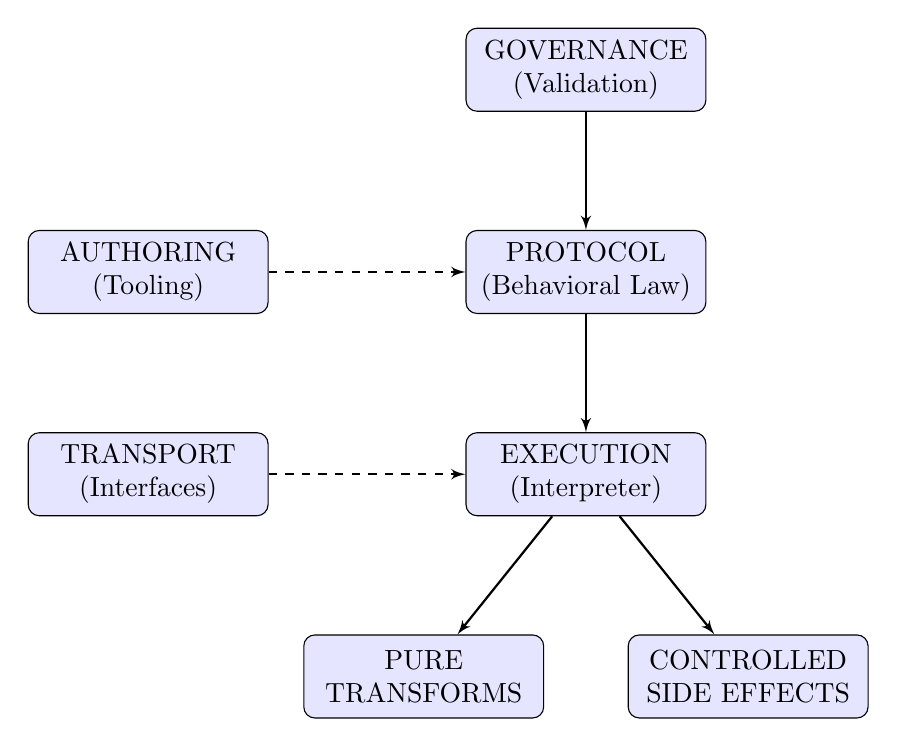
\begin{tikzpicture}[
    node distance=1.5cm,
    auto,
    block/.style={
        rectangle,
        draw,
        fill=blue!10,
        text width=8em,
        text centered,
        rounded corners,
        minimum height=3em
    },
    line/.style={
        draw, -latex', thick
    },
    dashedline/.style={
        draw, -latex', dashed, thick
    }
]

    % Nodes
    \node [block] (gov) {GOVERNANCE \\ (Validation)};
    \node [block, below=of gov] (proto) {PROTOCOL \\ (Behavioral Law)};
    \node [block, below=of proto] (exec) {EXECUTION \\ (Interpreter)};

    \node [block, below left=1.5cm and -1cm of exec] (pure) {PURE \\ TRANSFORMS};
    \node [block, below right=1.5cm and -1cm of exec] (side) {CONTROLLED \\ SIDE EFFECTS};

    \node [block, left=of proto, xshift=-1cm] (auth) {AUTHORING \\ (Tooling)};
    \node [block, left=of exec, xshift=-1cm] (trans) {TRANSPORT \\ (Interfaces)};

    % Edges
    \path [line] (gov) -- (proto);
    \path [line] (proto) -- (exec);
    \path [line] (exec) -- (pure);
    \path [line] (exec) -- (side);

    \path [dashedline] (auth) -- (proto);
    \path [dashedline] (trans) -- (exec);

\end{tikzpicture}
\caption{The Seven-Concern Architectural Model. Solid lines indicate runtime dependencies; dashed lines indicate design-time or interface interactions.}
\label{fig:arch_model}
\end{figure}

\subsection{Governance Layer}

Defines constitutional constraints and conformance rules. Governance validates protocols but does not execute them.

\subsection{Protocol Layer}

Pure declarative artifacts describing system behavior. No executable logic exists at this layer.

\subsection{Execution Layer}

Interprets protocols deterministically. Multiple implementations may exist, provided they satisfy conformance requirements.

\subsection{Capability Transformations}

Pure functions with no side effects. Identical inputs always produce identical outputs.

\subsection{Controlled Side Effects}

Explicitly declared mutations or external interactions. Effects are observable and ordered according to protocol semantics.

\subsection{Transport and Authoring}

Transport adapters expose execution via interfaces. Authoring tools assist protocol creation and validation but are never part of runtime execution.

\section{Case Studies (Abstracted)}

\subsection{Cryptographic Workflow System}

A prototype system implements hierarchical cryptographic workflows entirely through protocol artifacts. Deterministic transforms handle key derivation; controlled side effects persist metadata.

Execution traces verify identical outcomes across multiple engine strategies.

\subsection{Immutable Append-Only System}

An append-only system demonstrates protocol-governed state evolution. Integrity is enforced through declarative constraints rather than storage mechanics.

System state is derivable solely through event replay.

\subsection{Protocol Evolution Without Implementation Change}

Behavioral changes are introduced through new protocol versions while execution engines remain unchanged. Legacy and new behavior coexist without refactoring.

\section{Evaluation}

\subsection{Determinism Verification}

Repeated executions with identical inputs produce equivalent traces across engine variants, validating deterministic guarantees.

\subsection{Auditability Assessment}

Domain experts can determine system behavior by inspecting protocol artifacts alone, without code inspection.

\subsection{Implementation Replaceability}

Execution strategies can change without behavioral re-certification, provided conformance verification succeeds.

\section{Related Work}

Workflow engines govern sequencing, not semantics \cite{vanderAalst2003workflow}.
Low-code platforms abstract coding without governable behavior \cite{waszkowski2019lowcode}.
Formal methods specify behavior but do not govern execution \cite{lamport2002specifying}.
Microservices distribute implicit behavior across components \cite{newman2015building, fowler2014microservices}.

Protocol-governed architecture unifies specification and execution under a single authoritative model.

\section{Discussion}

\textbf{Limitations}

The approach is best suited for systems requiring explicit governance, auditability, and long-term behavioral stability. It is less appropriate for exploratory or highly non-deterministic domains.

\textbf{Future Work}

\begin{itemize}
\item formal engine verification,
\item standardized conformance suites,
\item protocol authoring tooling,
\item potential standards development.
\end{itemize}

\section{Conclusion}

As AI accelerates code generation, implicit system behavior becomes untenable. Protocol-governed architecture provides a path toward software systems whose behavior remains explicit, deterministic, and governable across implementation change.

By separating behavioral intent from execution mechanics, systems can evolve without losing meaning---addressing a fundamental challenge in modern software engineering.

\section*{Author Information}

\textbf{Bachi}\\
\emph{Contact:} \href{mailto:bachi.bachi@myyahoo.com}{bachi.bachi@myyahoo.com}

\vspace{1em}
\noindent \textbf{Conflict of Interest:} The author is developing commercial implementations of the described architecture.

\begin{thebibliography}{9}

\bibitem{newman2015building}
Sam Newman.
\textit{Building Microservices: Designing Fine-Grained Systems}.
O'Reilly Media, Inc., 2015.

\bibitem{vanderAalst2003workflow}
Wil M.P. van der Aalst, Arthur H.M. ter Hofstede, Bartek Kiepuszewski, and Alistair P. Barros.
Workflow patterns.
\textit{Distributed and Parallel Databases}, 14(1):5--51, 2003.

\bibitem{lamport2002specifying}
Leslie Lamport.
\textit{Specifying Systems: The TLA+ Language and Tools for Hardware and Software Engineers}.
Addison-Wesley Professional, 2002.

\bibitem{waszkowski2019lowcode}
Robert Waszkowski.
Low-Code Platform: A Revolution in Software Development?
In \textit{International Conference on Computational Collective Intelligence}, pages 299--310. Springer, 2019.

\bibitem{fowler2014microservices}
Martin Fowler and James Lewis.
Microservices: a definition of this new architectural style.
\textit{Martin Fowler}, 2014.
\url{https://martinfowler.com/articles/microservices.html}

\end{thebibliography}

\end{document}